%!TEX root = /Users/admin/Desktop/Documents/Academic/MA 470 -THESIS/THESIS/thesis.tex
\chapter{Introduction}
	Computer Scientists have long been interested in algebraic models are capable of describing computation by formulating a `program' as an algebraic expression along with a set of rules for reducing such expressions - ie `running' them.  The advantage of such algebras are that can be studied using formal reasoning techniques.  This means that we can prove things about them, and it also means that we can derive useful observations `programming' in them without actually ever having to go and implement them on a system.  Of course, these algebra often are used in real languages whether faithfully or as inspiration, but this is usually after they have been studied in detail for some time and we can be sure of their value.
	
	In the 1930's, Alonzo Church and Stephen Kleene introduced one such algebra, known as the $\lambda$-calculus.  In the $\lambda$-calculus, we can write programs as expressions that are a series of nested functions, and we can run these programs by invoking the functions within.  For example, the following is a very simple `successor' program that takes in a number $x$ and adds 1 to it, returning the result:
	\[
		(\lambda x. x + 1)
	\]
To run this program, we need to actually apply it to something - that is, we need to give it input.  We express this by placing the input to the right of the function, as in:
\[
	(\lambda x. x + 1) 4
\]
The above program first substitutes 4 in for the input $x$, yielding 4+1.  The program then returns the result, 5.  Since we can nest functions, a slightly more complicated version adds 1 to the input 4 and then multiplies the result by 3.  We give this program with each computational `step' below:
\begin{align*}
	(\lambda y. y * 3) ((\lambda x. x + 1) 4)
	(\lambda y. y * 3) (4+1)
	(\lambda y. y * 3) 5
	5 * 3
	15
\end{align*}
You are probably already getting a sense of theo expressive power of the $\lambda$-calculus.  In fact, it is capable of expressing any algorithm, even without the numbers and arithmetic operators we have implicitly included above!  Besides allowing the proof of many important results in computer science, the $\lambda$-calculus went on to inspire many programming languages like Lisp, ML and Haskell, and even some functionality in languages like Smalltalk, Ruby and Python.

However, the discover of the $\lambda$-calculus did not end the search for new algebra.  More recently, new kinds of programs and demands have emerged with the computational platform of \defmargin{distributed systems}.  These systems consist of loose networks of machines capable of exchanging messages and information.  We say this shared information and computational power belongs to `the system' in that it can be accessed from any system, and that any program running on the system can freely access these resources and generally behaves just as it would running on a single machine.

For example, consider the familiar system that powers your mobile phone network.  There may be one or more connected central servers, all of which are connected to the various towers that provide service.  Towers and servers may have different capabilities and responsibilities, but the important thing is that the entire system needs to behave as a single unit with a bunch of shared information and computational power.  A call in progress, for example, is a resource that will need to be accessed in various ways in the system - by a tower to handle the call, by a server, perhaps, to handle the billing and routing of that call.  Mobile clients are also connected and a part of this system.  When a user places a call, for example, he may use some capabilities on the phone to input the number, which is then transmitted by the phone to the tower, which is sent to the server to be routed.  This entire `program' for making a call is one seamless operation that is happening across several machines.  

\begin{figure}[H]
\centering
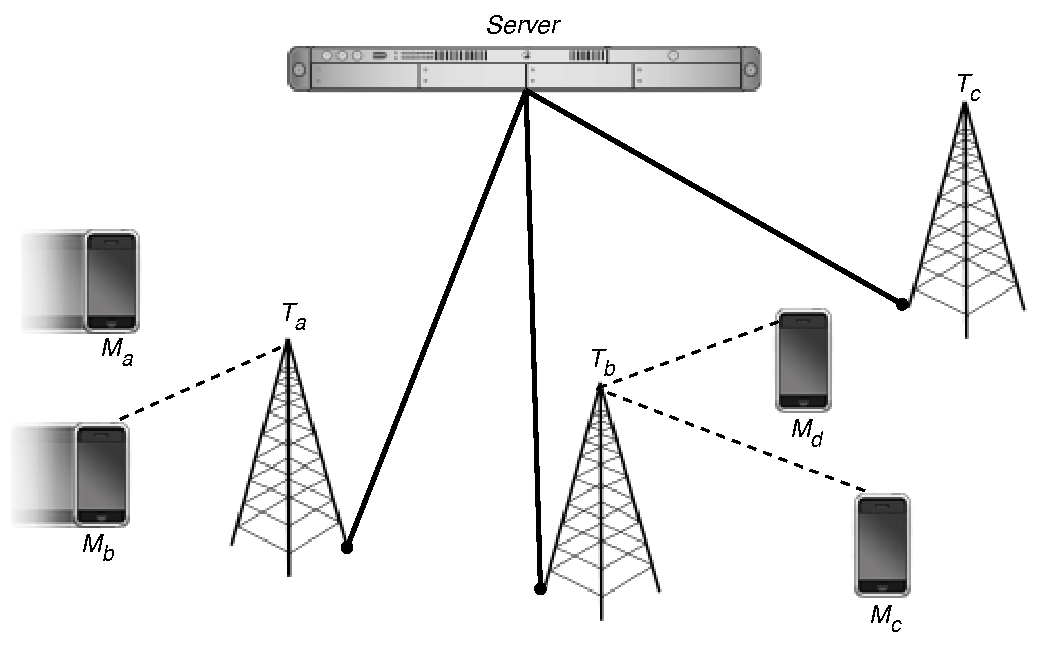
\includegraphics[scale=0.7]{figures/cell_network.pdf} % requires the graphicx package
\caption{A Distributed Mobile System}
\label{fig_cell_network}
\end{figure}

The demands of a distributed system strain the expressive power of the $\lambda$-calculus.  Since all computation is modeled as a function, our only way to model a resource is as a function.  However, functions can only be accessed directly -- input can only come by directly apply the function to that input.  If we want access to a resource on a system, we might not know where it is or what it is doing.  Furthermore, our system of many machines could be doing many different things at once: routing calls, handling other calls in session, calculating a bill.  Yet the $\lambda$-calculus has no means of easily expressing the concurrency which is so basic to many distributed systems.


Consider the phones on our system.  They are \emph{mobile} - in the sense that their connections to the system can be added and removed at any time.  In the \reffig{fig_cell_network} above, client $M_b$ is wirelessly connected to tower $T_a$ while $M_c,M_d$ are connected to $T_b$.  Client $M_a$ is currently disconnected and $T_c$ has no clients.  All the towers maintain a hard-wired link to $server$.  We refer to the connections in a distributed system as its communication \defmargin{topology}.

In \reffig{fig_cell_network}, $M_a$ and $M_b$ are in physical movement, so they their connections may change soon.  $M_b$ might, for example, go out of range and disconnect from $T_a$ and connect to $T_b$ instead.  Such changing communication topologies presents even more difficulties to the $\lambda$-calculus.  How can we abstract function invocation such that a function can be called from one place at one time, and another place later?  Even if we could some how invoke a function indirectly, how could we deal with the fact that a function (say a client's ability to receive a call) is not currently available?

Clearly we need an algebraic model for computation eases the difficulty of modeling such systems.  Such a model might consider computation via its natural distributed unit - the process.  A process is just a computational task.  Since concurrency is such a natural operation, we make it a part of our algebra.  A system, then, is simply a group of processes which are executing concurrently. The important thing about processes is that they maintain computation state independently of one another.  Thus, instead of a single state of computation that has functions interacting via invocation, processes interact via \defmargin{message passing} -- sending data back-and-forth via named channels.  

Because these channels can be shared among processes and used an arbitrary number of times, there is not a concrete invocation system for a chunk of computation the way there is in a function - processes simply send values to channels, assuming the receiver (if there is one) will do something useful with it.  Any bit of functionality can be referred to as a process, but with no specification of the granularity.

A major step towards such an algebra came in the 1980's when Robin Milner introduced his Calculus of Communicating Systems (CCS).   The CCS modeled systems as groups of communicating processes interacting via shared channels, and drastically eased the difficulty of modeling indirectly invoked concurrent operations.  However, the CCS still would have had trouble with our mobile phone network, because it did not provide a way for processes to gain and loose their communication channels.

	Although it can be defined in other ways, one of the ways of giving a process's \emph{location} is in terms of the communication channels which can be used to access it.  Since processes are the units populating the space of a CCS system, it is natural to think of a process's location in terms of the processes which are `near' it - those it can communicate with via channels.  In this case, changing the communication channel topology of a system changes the locations of its component processes.  
	
	In the CCS, channel topology is static - it does not allow new connections to be made or old ones to be removed.  Not long after CCS's birth, Robin Milner, Joachim Parrow and David Walker created an improved algebra called the \picalc.  The \picalc\ allows communication channels to be dynamically established and relinquished between processes.  Thus, it gives a kind of \emph{mobility} of processes, which vastly expands the capabilities of interaction in a system and finally allows us to give an account of our mobile phone system.
	
	As an example of how naturally the \picalc\ models distributed systems, let us again consider our mobile phone network\footnote{This presentation is adapted from a version first given in \cite{miln99}}.  \note{Jim: I choose to give this presentation synchronously with milner.  I think it could be adapted, but I'm hoping that this will be a natural way to see the expressive power of the synchronous algebra but still can motivate the asynchronous presentation by pointing out that it is the way real systems behave.  Also, it is simpler and (I think) thus a better introduction to the calculus.}  Our system will be simplified a bit: only two towers and one phone, with the only capabilities being talking on the phone or switching from one tower to another.
	
	First we give a process describing the behavior of a mobile phone:
	\[
		Mobile(talk, switch) \pdef \ssend{talk}{} Mobile(talk,switch) + \receive{switch}{t,s} Mobile(t,s)
	\]
	Above, we use $\pdef$ to mean that the term to the right of the $\pdef$ is given the shorthand $Mobile$ and that it uses the channels $talk$ and $switch$ given elsewhere.  The channels given in the parenthesis are simply substituted into the term on the right's corresponding channels.  Hence, for example, $Mobile(t,s)$ would be this right-hand term with the channels $t$ and $s$ substituted for $talk$ and $switch$. We call $Mobile(t,s)$ the \defmargin{interface} the right-hand term.
	
	The notation \ssend{talk}{} means that we are sending an inputless signal on channel $talk$, while $\receive{switch}{t,s}$ means we are listening on $switch$ and use the input $t,s$.  After a signal is sent or received on a channel, execution then continues with the term immediately to the right of the term, using the input provided (if any).  
	
	Thus, $\receive{switch}{t,s} Mobile(t,s)$ indicates that we should listen on $switch$ for the input $t,s$ and then use $t,s$ to `spawn' a new computation of $Mobile$ with these new channels. The term $\ssend{talk}{} Mobile(talk,switch)$ means send a signal on $talk$ before spawning a computation of $Mobile$ with the same $talk,switch$ channels we are using.  Finally, the $+$ operator denotes that we should choose to compute one or the other of the operands (but not both).  In sum then, our mobile process has the ability to either send along $talk$ and stay in its current location, or it can receive on $switch$ and `move' to the location where it has new talking and switching channels $t,s$.  This last capability expresses the mobile nature of our processes with surprising elegance: here we have just expressed that channels $talk,switch$ are lost and new channels $t,s$ are established.
	
	Next we consider the behavior of a tower:
	\begin{align*}
		ActiveT(talk,switch,gain,loose) \pdef & \receive{talk}{}ActiveT(talk,switch,gain,loose) \\  
		 & +\receive{loose}{t,s}\ssend{switch}{t,s}IdleT(gain, loose)\\
		IdleT(gain,loose) \pdef & \receive{gain}{t,s}ActiveT(t,s,gain,loose)\\
	\end{align*}
Here, the are two `states' our tower can be in.  It can be active in talking with a mobile phone, or it can be disconnected and idle.  If it is active, it can either receive on $talk$ (from the phone) and continue to be active, or it can receive on $loose$ (from the server, as we shall see below).  In the latter case it then sends $t,s$ on $switch$ before becoming idle.  That is, it will receive some new channels $t,s$ on $loose$ and then send them to the phone on $switch$ before becoming idle.  An idle tower has only one capability: to receive on $gain$ and then become active again on the new channels $t,s$.

Finally we give the behavior of the server:
\begin{align*}
	Server_1 \pdef \ssend{loose_1}{talk_2,switch_2} \ssend{gain_2}{talk_2,switch_2} Server_2\\
	Server_2 \pdef \ssend{loose_2}{talk_1,switch_1} \ssend{gain_1}{talk_1,switch_1} Server_1
\end{align*}
Above, the server has two states: it can be controlling tower 1 or it can be controlling tower 2.  In either case, the only capability is to loose one tower and gain the other before going into the opposite state.  Hence, in $Server_1$ we can send to the first tower on $loose_1$ and then to the second tower on $gain_2$ before entering state $Server_2$.

We have now completely described the components of our system, but we still haven't put them all together.  To do so, we'll need a new operator.  This operator denotes that its operands run concurrently in parallel and is denoted $\comp$.  Thus, our system is simply:
\begin{center}
	\small{$\textstyle Mobile(talk_1,switch_1)|ActiveT_1(talk_1,switch_1,gain_1,loose_1)|IdleT(gain_2,loose_2)|Server_1$}
\end{center}

	